\DailyTitle{6321 Log (October 18, 2010)}

\DailySection{Goals}

\begin{enumerate}
\item Vecbos candle data exercise: start after lunch!
\item Hcal DQM: finish the implementation of task module
\item Hcal noise: look at correlations between the three test variables
\item Hcal noise: have a preliminary version of presentation
\end{enumerate}

\DailySection{Summary List}

\begin{enumerate}
\item Sent out the \texttt{RooDataSet}s to people.
\item Looked at the correlations between test variables
\item Fixed a fatal error in the two-level fit.  Now the chi2 is always positive, and the result look a lot more like the linear fit
\item Made a preliminary version of the presentation.
\end{enumerate}

\DailySection{Note on progress during Sunday}

\begin{enumerate}
\item Started the leptoquark jobs.  Expect them to be finished soon.
\item Don't know how to run Will's code.  I will ask him later, but for the moment I'll write my own \texttt{RooDataSet} converter.
\item Successfully exported \texttt{RooDataSet}s for W, Z, $t\bar{t}$, single t (s, t, tW), QCD (ppMuX).
\end{enumerate}

\DailySection{Hcal noise test statistics correlation}

Correlation between linear fit vs. two-level fit, as well as linear fit vs. RMS-series are plotted.
The results between linear and two-level fits are shown in figures \ref{Figure_6321HTestStatisticsLinearVsTwoLevel}
and \ref{Figure_6321HTestStatisticsLinearVsTwoLevel100}.  Results between linear and combinations
of RMS8/9 and max charge/total charge are shown in figures \ref{Figure_6321HTestStatisticsLinearVsRMS8OverMaxCharge}
- \ref{Figure_6321HTestStatisticsLinearVsRMS9OverTotalCharge100}.

As we can see, the two level fit is highly correlated with linear fit, and we might not be able to gain much from this.
The RMS-series, however, picks out the spike ones and is a more natural handle to pick out those than the linear fit.
While linear fit could cut out the spike ones (if we squeeze the envelope enough....and also make it dependent on total charge),
the RMS-series can be complementary.
Overall the max charge make a better denominator, since the signal cluster is higher.
Comparing RMS8/Max (\ref{Figure_6321HTestStatisticsLinearVsRMS8OverMaxCharge100}) and RMS9/Max (figure \ref{Figure_6321HTestStatisticsLinearVsRMS9OverMaxCharge100}),
The signal is more concentrated in RMS9/Max, but there is a clearer noise region in RMS8/Max.
And RMS8/Max seems to have better separation between the signal cluster position and the lower wing of noise.

The scatter plot of (test statistics of) RMS8/Max vs. RMS9/Max (figures \ref{Figure_6321HTestStatisticsRMS8OverMaxVsRMS9OverMax} and
\ref{Figure_6321HTestStatisticsRMS8OverMaxVsRMS9OverMax100}) show that RMS8/Max seems to be a better one to use.

\begin{figure}[h]
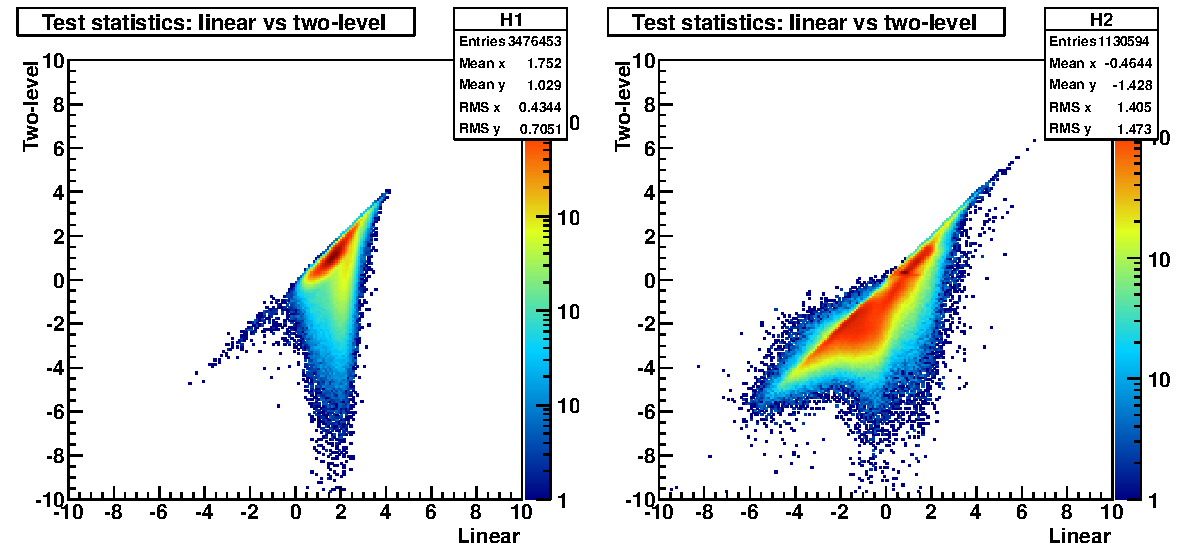
\includegraphics[width=120mm]{DailyLog/6321/6321HTestStatisticsLinearVsTwoLevel.pdf}
\caption{Test statistics of linear fit vs. two-level fit.  Left: signal, right: noise}
\label{Figure_6321HTestStatisticsLinearVsTwoLevel}
\end{figure}

\begin{figure}
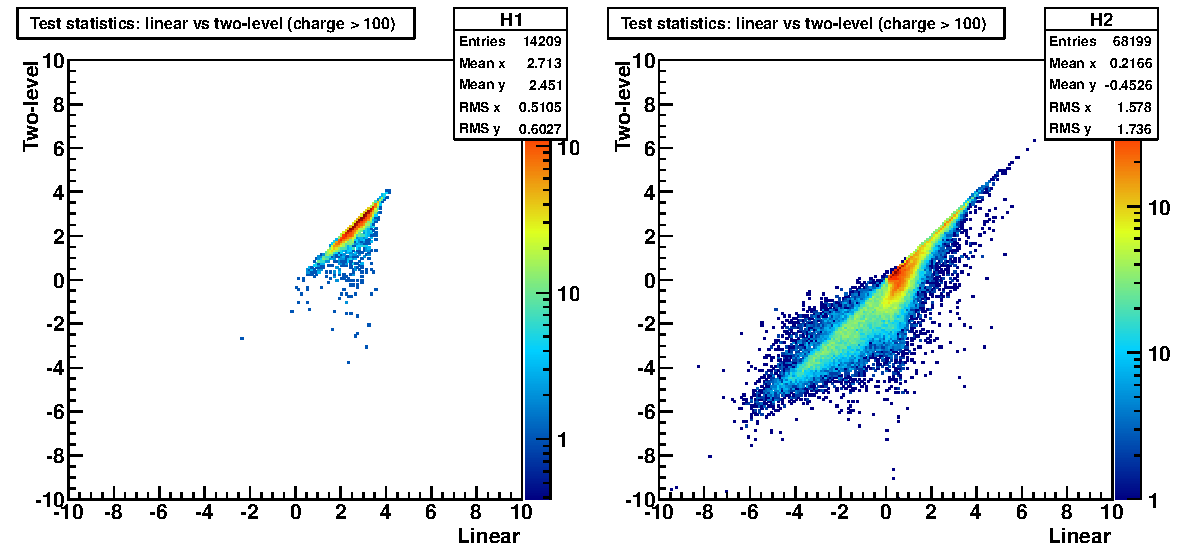
\includegraphics[width=120mm]{DailyLog/6321/6321HTestStatisticsLinearVsTwoLevel100.pdf}
\caption{Test statistics of linear fit vs. two-level fit, charge \textgreater 100.  Left: signal, right: noise}
\label{Figure_6321HTestStatisticsLinearVsTwoLevel100}
\end{figure}

\begin{figure}
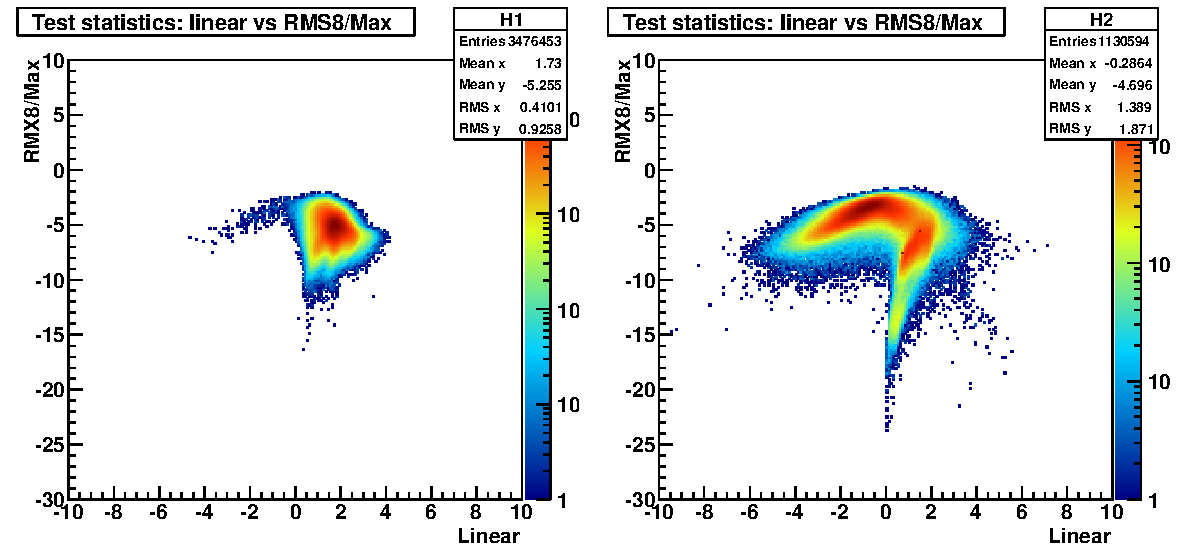
\includegraphics[width=120mm]{DailyLog/6321/6321HTestStatisticsLinearVsRMS8OverMaxCharge.pdf}
\caption{Test statistics of linear fit vs. RMS8/max charge.  Left: signal, right: noise}
\label{Figure_6321HTestStatisticsLinearVsRMS8OverMaxCharge}
\end{figure}

\begin{figure}
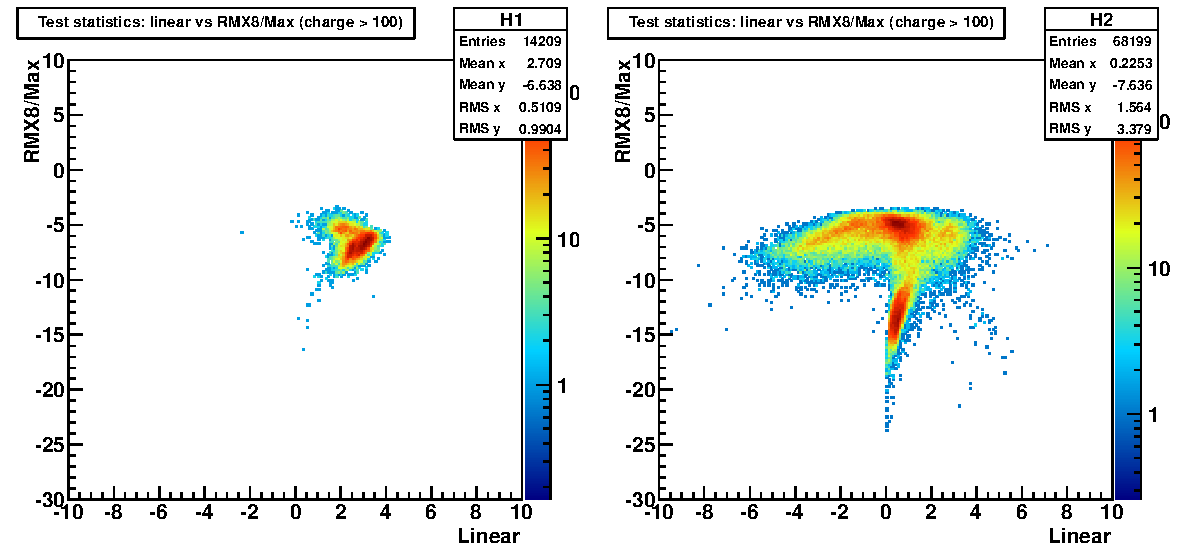
\includegraphics[width=120mm]{DailyLog/6321/6321HTestStatisticsLinearVsRMS8OverMaxCharge100.pdf}
\caption{Test statistics of linear fit vs. RMS8/max charge, charge \textgreater 100.  Left: signal, right: noise}
\label{Figure_6321HTestStatisticsLinearVsRMS8OverMaxCharge100}
\end{figure}

\begin{figure}
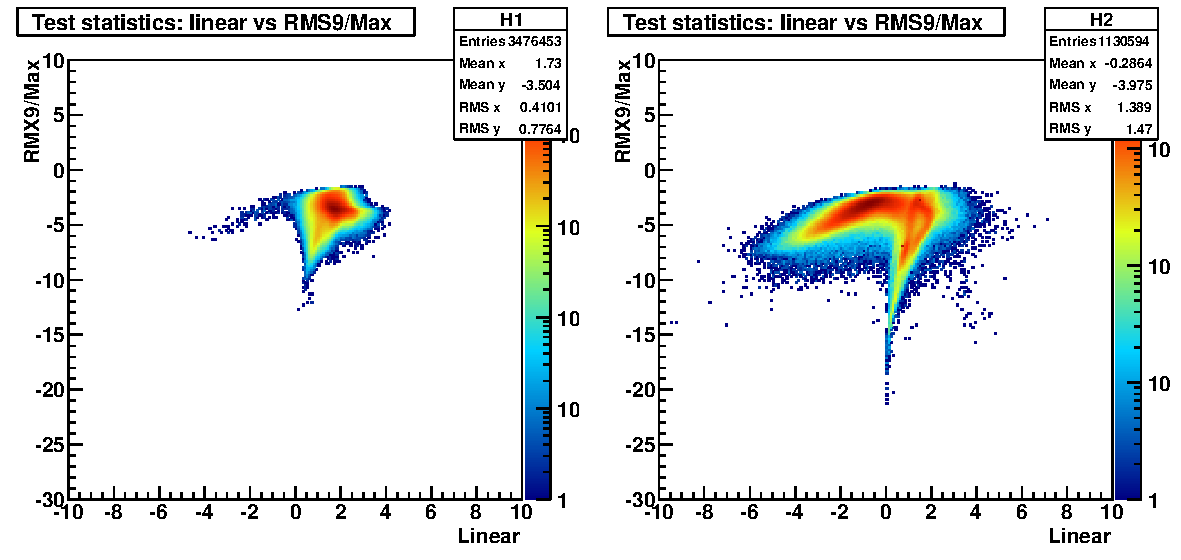
\includegraphics[width=120mm]{DailyLog/6321/6321HTestStatisticsLinearVsRMS9OverMaxCharge.pdf}
\caption{Test statistics of linear fit vs. RMS9/max charge.  Left: signal, right: noise}
\label{Figure_6321HTestStatisticsLinearVsRMS9OverMaxCharge}
\end{figure}

\begin{figure}
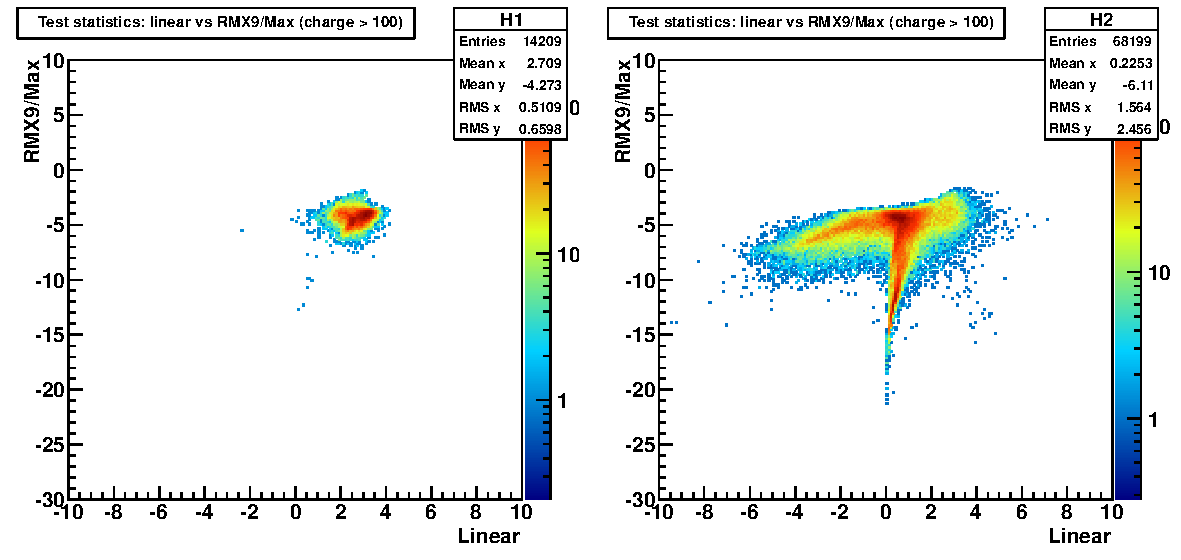
\includegraphics[width=120mm]{DailyLog/6321/6321HTestStatisticsLinearVsRMS9OverMaxCharge100.pdf}
\caption{Test statistics of linear fit vs. RMS9/max charge, charge \textgreater 100.  Left: signal, right: noise}
\label{Figure_6321HTestStatisticsLinearVsRMS9OverMaxCharge100}
\end{figure}

\begin{figure}
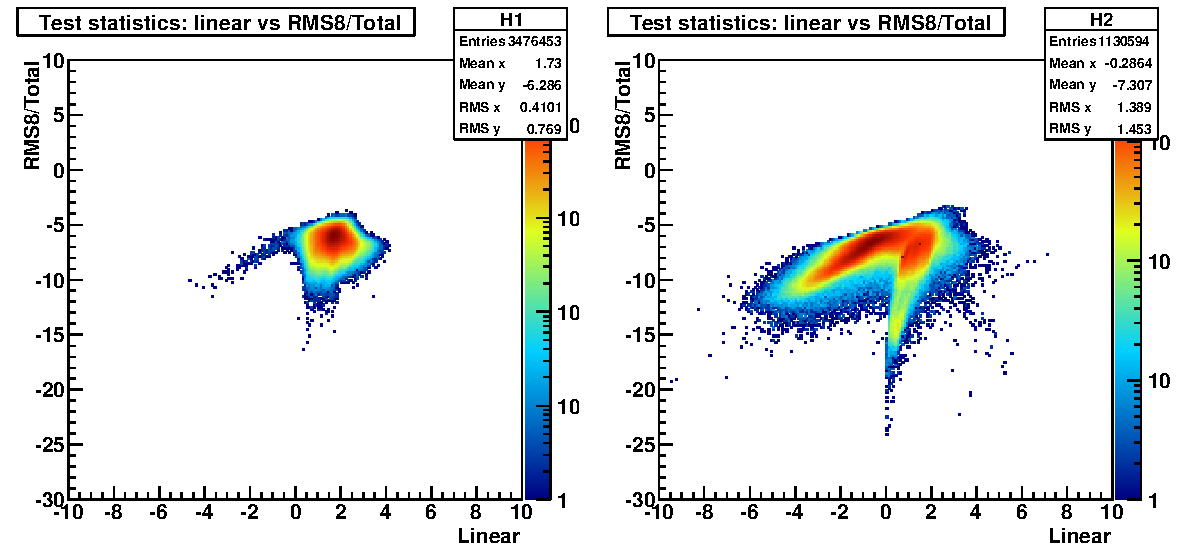
\includegraphics[width=120mm]{DailyLog/6321/6321HTestStatisticsLinearVsRMS8OverTotalCharge.pdf}
\caption{Test statistics of linear fit vs. RMS8/total charge.  Left: signal, right: noise}
\label{Figure_6321HTestStatisticsLinearVsRMS8OverTotalCharge}
\end{figure}

\begin{figure}
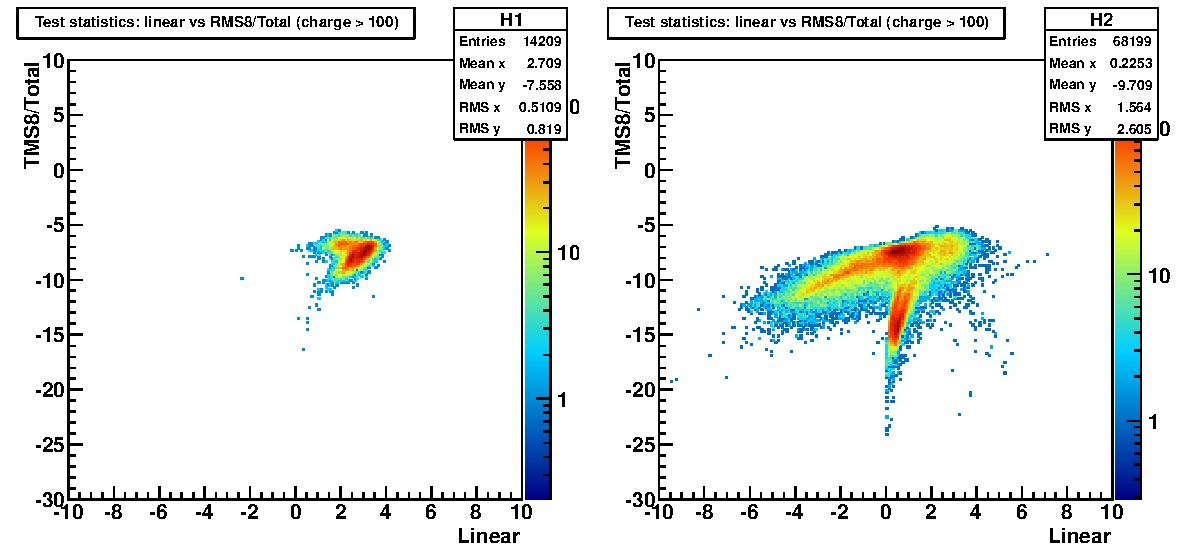
\includegraphics[width=120mm]{DailyLog/6321/6321HTestStatisticsLinearVsRMS8OverTotalCharge100.pdf}
\caption{Test statistics of linear fit vs. RMS8/total charge, charge \textgreater 100.  Left: signal, right: noise}
\label{Figure_6321HTestStatisticsLinearVsRMS8OverTotalCharge100}
\end{figure}

\begin{figure}
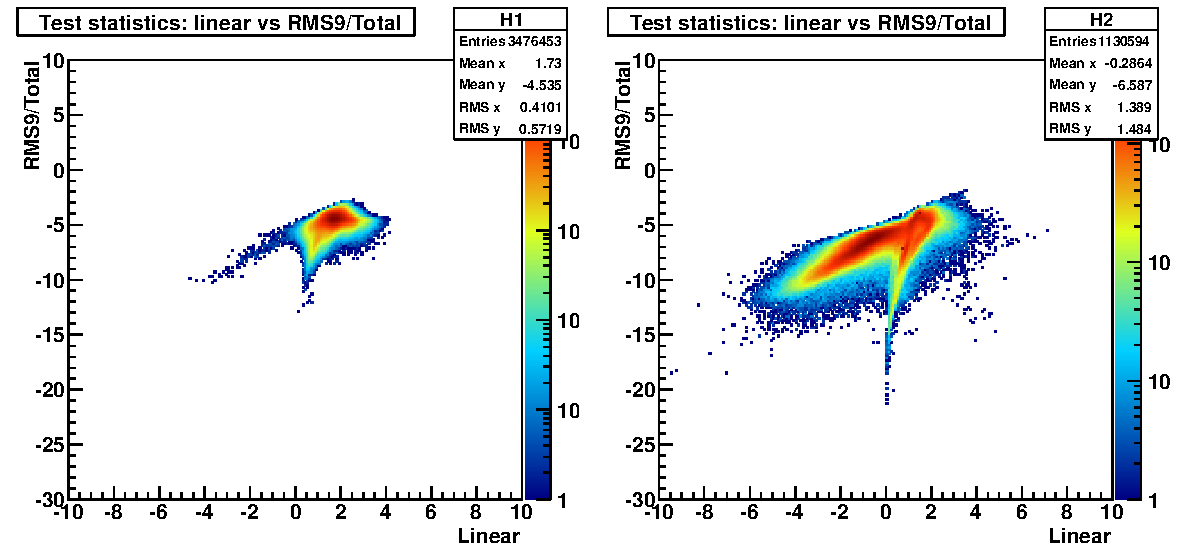
\includegraphics[width=120mm]{DailyLog/6321/6321HTestStatisticsLinearVsRMS9OverTotalCharge.pdf}
\caption{Test statistics of linear fit vs. RMS9/total charge.  Left: signal, right: noise}
\label{Figure_6321HTestStatisticsLinearVsRMS9OverTotalCharge}
\end{figure}

\begin{figure}
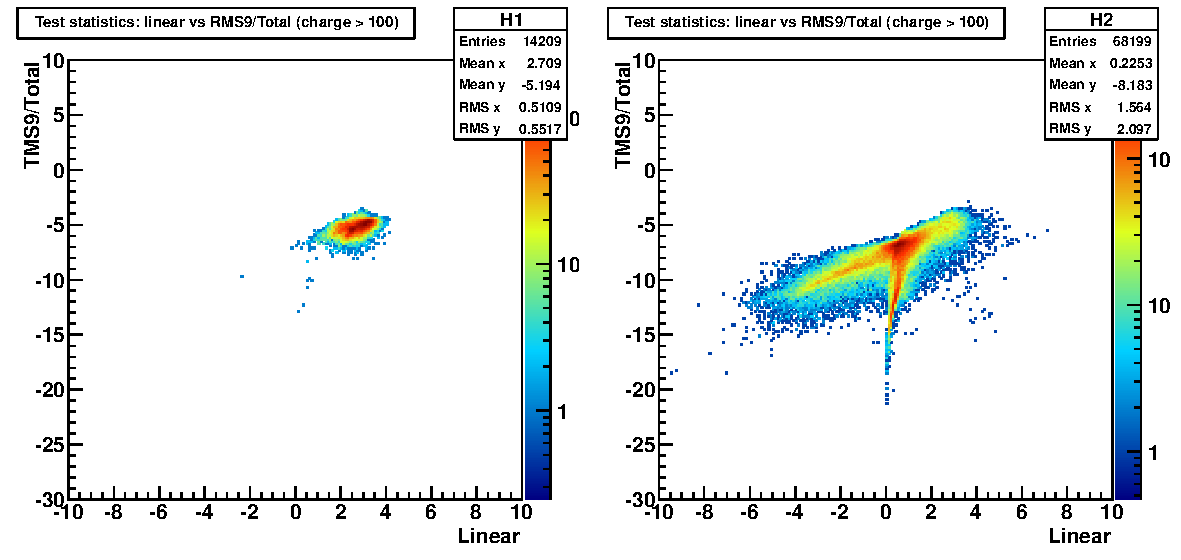
\includegraphics[width=120mm]{DailyLog/6321/6321HTestStatisticsLinearVsRMS9OverTotalCharge100.pdf}
\caption{Test statistics of linear fit vs. RMS9/total charge, charge \textgreater 100.  Left: signal, right: noise}
\label{Figure_6321HTestStatisticsLinearVsRMS9OverTotalCharge100}
\end{figure}

\begin{figure}
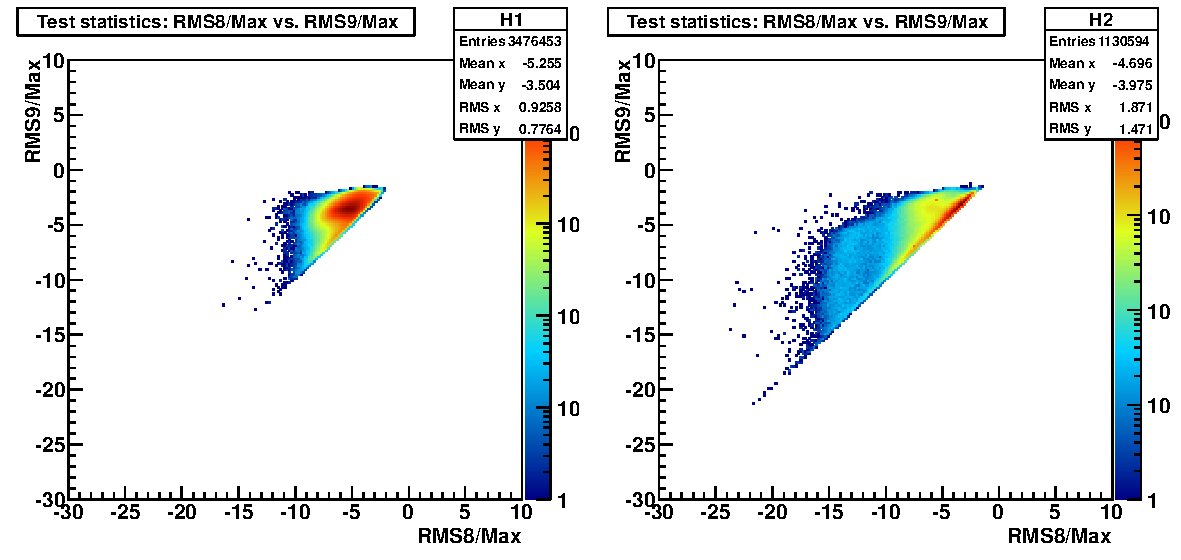
\includegraphics[width=120mm]{DailyLog/6321/6321HTestStatisticsRMS8OverMaxVsRMS9OverMax.pdf}
\caption{Test statistics of RMS9/max and RMS8/max.  Left: signal, right: noise}
\label{Figure_6321HTestStatisticsRMS8OverMaxVsRMS9OverMax}
\end{figure}

\begin{figure}
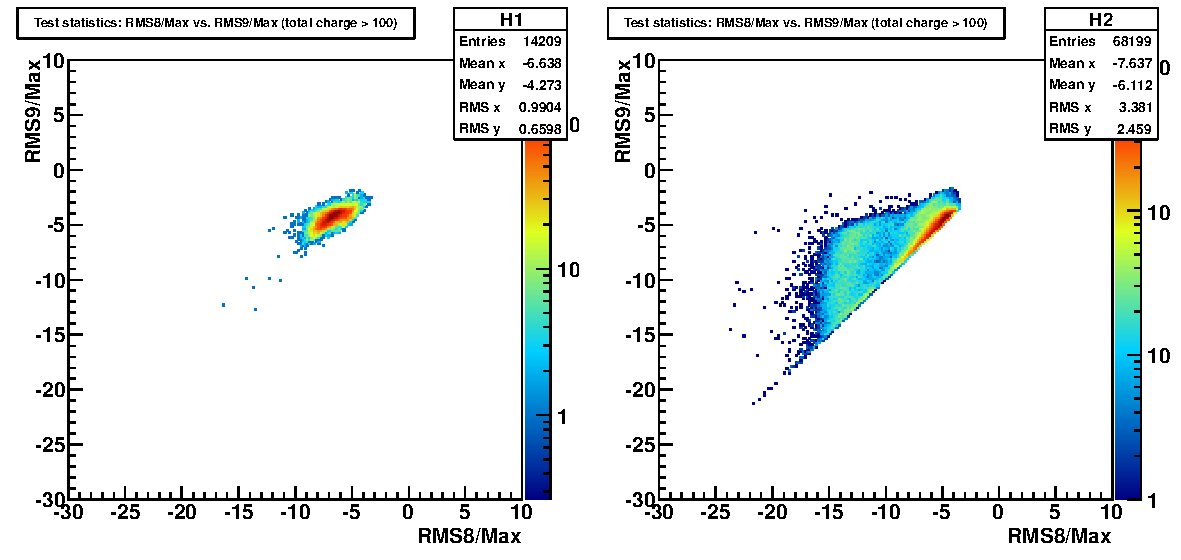
\includegraphics[width=120mm]{DailyLog/6321/6321HTestStatisticsRMS8OverMaxVsRMS9OverMax100.pdf}
\caption{Test statistics of RMS9/max and RMS8/max, charge \textgreater 100.  Left: signal, right: noise}
\label{Figure_6321HTestStatisticsRMS8OverMaxVsRMS9OverMax100}
\end{figure}

\DailySection{Vecbos candle data exercise}

Start at 12:34 computer time.  Goal is to produce all plots/tables used in the notes that are related to data as soon as possible.
Hopefully I can get all of them done in one afternoon.  While it is running, let me compile a list of plots/tables/numbers to produce.

\begin{enumerate}
\item Fit with tight isolation and extract $\alpha_L$.  Compare with normal isolation cut.
\item Simultaneous fit
\item Data extracted yields
\item Get the ratio from the yields
\item Redo fit with different jet threshold and produce JES uncertainty estimate
\item Anti-isolation to produce QCD control shape
\item Check basic plots to see if everything looks roughly okay.
\end{enumerate}

Now it's 14:27.  I'm still submitting jobs.  :(
Splitting jobs in smaller segments makes it a lot faster.
14:43.  Jobs done.  Finished submitting job at 14:31.
It takes about 20 minutes to submit all jobs, so....the total turnaround time on my side is about 30 minutes for around 3/pb.
Copying takes a while though...  15:18.  Finished copying.

The fits to MC signal sample takes a lot of time.  Don't redo it again when data come.
Todo item #1: make a script to output the fit result tables directly.  For now let me proceed.
Signal inclusive fits finish in a flash.  Todo item #2: make a script to output the fit result lables.
The JES fits are also really fast.  Todo item #3: ditto.
Todo item #4: setup script to produce the ratio.

Uhm....all the scripts run fine....
So I only need to write scripts to generate tables in latex format and I'm done with data part of the note (also to get the ratio).
Tomorrow let me do a MC rush to generate all MC plots/tables.


\DailySection{Reflection}

\DailySection{Goals for next work day}

\begin{enumerate}
\item Eat lunch
\item Eat dinner
\item Find the red herring
\end{enumerate}



